If the LHC is operated at the design bunch spacing of $\unit{25}{\nano\second}$, bunch crossings occur with a rate of about $\unit{40}{\mega\hertz}$. This rate has been reduced by at least factor of two during Run I of the LHC because of the increased bunch spacing. Still, event rates of this magnitude can not be handled by the available means of data processing. The total event rate is therefore reduced by a factor of about $10^6$ by two subsequent trigger systems. The Level-1 (L1) trigger consists of programmable electronics, allowing for a fast primitive reconstruction of physics objects in the calorimeters and the muon system. This system reduces the event rate to a maximum of $\unit{100}{\kilo\hertz}$. Following an L1 accept (L1A), the CMS data acquisition system (DAQ) collects the event information from the readout of the different subdetectors and passes it on to the High-Level trigger (HLT). The HLT is a software trigger and has access to the full detector readout~\cite{Adam:2005zf}. It can perform a full reconstruction of the events using similar algorithms used in offline data analysis. It accepts events at a rate of a few $\unit{10^2}{\hertz}$.  

\subsubsection*{Level-1 trigger (L1)}
The outputs of the different subdetectors are stored in pipelined buffers inside the readout electronics. This limits the time between the bunch crossing and the distribution of the L1A to the subsystems to $\unit{3.2}{\micro\second}$. The L1 is therefore constructed from mostly custom-built programmable electronics either directly inside the detector or located close by in the underground facilities. As the readout of the tracker and track reconstruction are not feasible on this time scale, only calorimeter and muon system information are used. The L1 system is divided into local, regional and global components, as shown in Figure~\ref{fig:L1Daq}. 

In the calorimeter trigger the local components are the trigger primitive generators (TPGs). For $\vert \eta \vert \leq 1.74$ they have an ($\eta,\phi$)-coverage of 0.087$\times$0.087, corresponding to one HCAL tower and a 5$\times$5 matrix of ECAL crystals in front of it. The TPGs communicate the energy deposits in the trigger tower and the number of the bunch crossing to the regional calorimeter trigger. One calorimeter region consists of 4$\times$4 trigger towers. Candidates for electrons or photons (e/$\gamma$) are formed by by selecting the towers with the highest $E_T$ in the ECAL. Based on information about the energy distribution inside the ECAL tower, the ratio of energy in ECAL and HCAL in the trigger tower and the overall distribution of energy in the neighbouring trigger towers the candidates are classified as isolated or non-isolated. Per region, four isolated and four non-isolated e/$\gamma$ candidates and the transverse energy sums of the trigger towers are passed to the global calorimeter trigger (GCT). Additionally, information for $\tau$ and muon identification is provided. The GCT performs a simple jet clustering algorithm and is able to calculate per event observables such as the number of jets, the total and missing transverse energy, and sum of the transverse energy of all jets above a certain threshold ($H_{\mathrm{T}}^{\mathrm{L1}}$). These information are delivered to the global trigger

In the muon trigger all three detector components (DT,CSC, and RPC) are used. In the local trigger, the DT chambers deliver track segments in the $\phi$-projection and hit patterns in the $\eta$-projection, while the CSCs produce three-dimensional track segments. Both use timing information to associate this information with the bunch crossing. In the regional trigger, DT and CSC information are processed in separate track finders, which produce muon candidates. These are ordered as a function of \pt and track quality and up to four candidates are delivered to the global muon trigger from each track finder. The RPCs also deliver muon candidates. With their excellent timing resolution of about $\unit{1}{\nano\second}$ they deliver an unambiguous association of the muon candidates to the correct bunch crossing. The global muon trigger receives up to four muon candidates each from the DTs, the CSCs, and the barrel and endcap RPCs. The information consists of \pt, $\eta$, $\phi$, and information on the quality of the muon reconstruction. Candidates from the RPCs are matched with the ones from DT and CSC and, if matches are found, merged into single candidates. Unmatched candidates with low quality are suppressed. The track of the candidates is extrapolated back into the calorimeters to add the minimum ionising particle signature and isolation information from the regional calorimeter trigger. The four best muon candidates are forwarded to the global trigger. 

The global trigger collects the information from the global muon and calorimeter triggers. Up to 128 trigger algorithms can be performed on the trigger objects at the same time, the most basic being simple \pt thresholds. If the criteria of one of the algorithms is met by the event, it is accepted by the L1 trigger and the L1A is sent to the DAQ to read out the event.  


\subsubsection*{Data acquisition system (DAQ)}
Following an L1A the DAQ receives the information from the different subdetectors split in about 650 data sources, each delivering about 2\,kB of data. These event fragments are assembled into whole events by the event builder. The event is then sent to one Filter Unit in the Event Filter, where the HLT software is running. The DAQ has to deal with input rates of up to $\unit{100}{\kilo\hertz}$ and consists of 8 nearly independent slices, each able to take input at a rate of $\unit{12.5}{\kilo\hertz}$. The DAQ includes a back-pressure system, which automatically throttles the L1 trigger in case the input rate exceeds the capability of the DAQ . This introduces dead times in the detector readout but prevents data corruption and buffer overflows. To fully utilise the capacities of the trigger system and the DAQ, trigger thresholds can be adapted during data taking. The shortest time scale on which the thresholds are kept constant is called lumi section and is defined as $2^{20}$ LHC orbits, corresponding to about $\unit{93}{\second}$. The structure of the DAQ is shown in Figure~\ref{fig:L1Daq}.
\begin{figure}[htbp]
\centering
\begin{minipage}[t]{0.49\textwidth}
  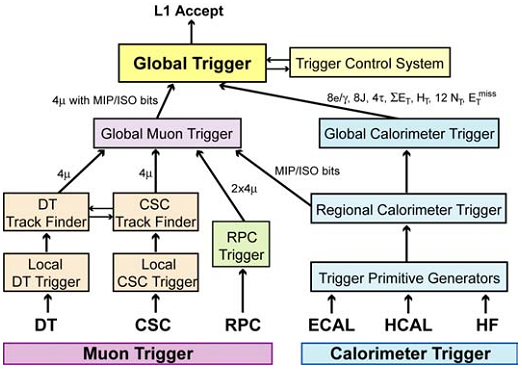
\includegraphics[width=\textwidth]{plots/CMS/L1Schema.png}
\end{minipage}
\begin{minipage}[t]{0.49\textwidth}
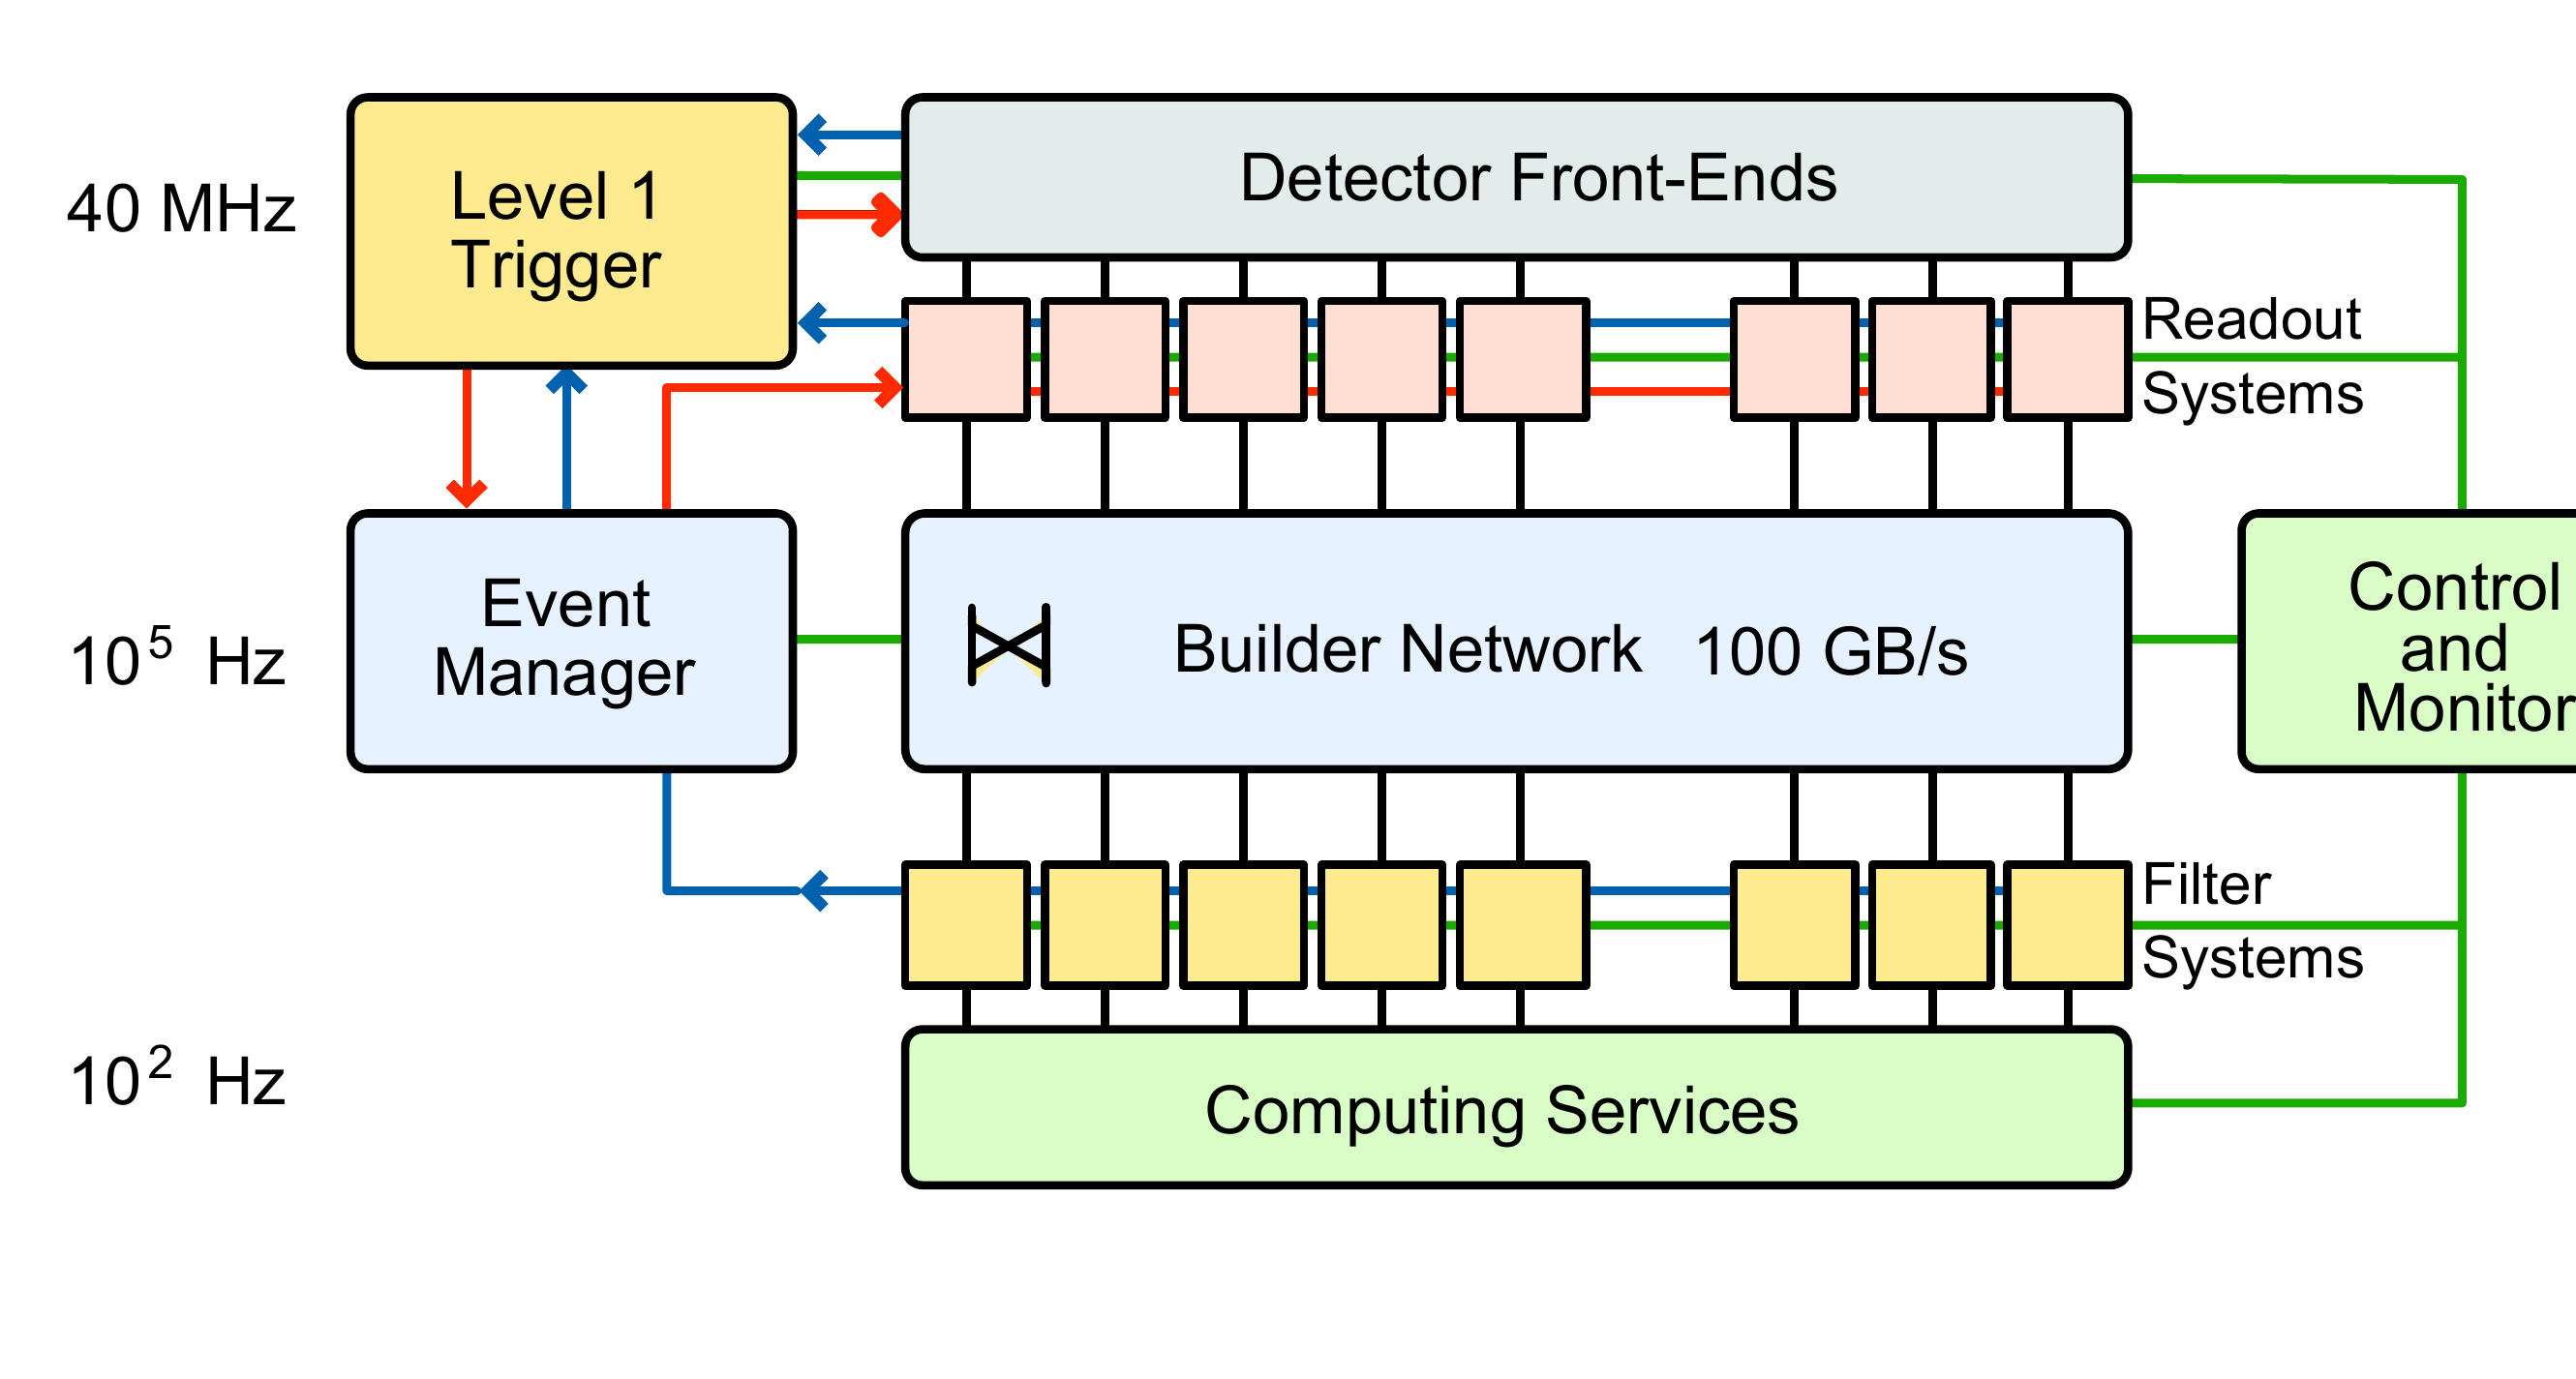
\includegraphics[width=\textwidth]{plots/CMS/DAQ.png}
\end{minipage}
\caption{Structure of the CMS Level-1 trigger (left) and data acquisition system (DAQ) (right)}
\label{fig:L1Daq}
\end{figure}

\subsubsection*{High level trigger (HLT)}
The HLT software is run on a dedicated computing element, the event filter farm, located in the CMS service caverns. During the data taking in 2012 it consisted of about 13200 processor cores~\cite{HLTProceedings}, allowing for a processing time of about $\unit{150}{\milli\second}$ at a input rate of $\unit{100}{\kilo\hertz}$. The HLT system reduces input data rates of up to $\unit{100}{\giga\byte\per\second}$ to several $\unit{\text{hundred}}{\mega\byte\per\second}$, which are sent to the CERN computer centre for storage. As a full event reconstruction can be performed at HLT level, even if it is often restricted to small regions of the detector for timing reasons, much more complex quantities can be used to separate potentially interesting signatures from the large backgrounds. However, approximate methods have to be used sometimes to maintain an acceptable processing time per event. Also, some calibration and alignment methods can only be performed after the data taking, making the HLT less precise compared to the offline reconstruction. While a large variety of triggers is used by CMS to select different kinds of events, this description will focus on the ones most relevant to this analysis. 

The most important signal and control samples for this analysis are collected with dilepton triggers. In general, they select events that contain two leptons (electrons or muons), of which one is required to have a reconstructed transverse momentum \pt of at least $\unit{17}{\giga\electronvolt}$, while for the second this threshold is relaxed to $\unit{8}{\giga\electronvolt}$. In general, the lepton with the higher (lower) \pt is referred to as the leading (trailing) lepton.  For muons, simply the presence of an reconstructed muon with a given \pt threshold is required. For electrons additional identification and isolation requirements are applied to keep the trigger rates at a acceptable level. For the most part, the algorithms employed to reconstruct muons and electrons are the same among all possible combinations of leptons. However, for $\mu\mu$ events an additional trigger, which uses tracker information for the trailing muon, is available, increasing the efficiency in this channel. The triggers used for preselection at L1 level also differ in their thresholds~\cite{HLTConfigBrowser} between the different lepton combinations. As the algorithms to reconstruct physics objects at HLT level are so similar to those used offline, no dedicated description is given here. An overview over the exact trigger definitions is given in in appendix~\ref{app:trigger}.

Other HLT paths used in this analysis select events based on the scalar sum of the \pt of hadronic jets (\HT), the $\alpha_{\mathrm{T}}$ variable~\cite{Khachatryan2011196}, which takes into account balance of jets in an event, and single electrons and muons, which are selected with tighter identification and isolation criteria compared to the dilepton triggers. Also, in order to study non-prompt leptons, events with low \pt single leptons are selected using trigger paths that apply the same selection as the different legs of the dilepton triggers.  

As the trigger rates for the \HT, $\alpha_{\mathrm{T}}$, and low \pt single lepton triggers are very high, these triggers are prescaled, meaning that only a predefined fraction of the selected events are actually recorded and reconstructed.

  


